% Options for packages loaded elsewhere
\PassOptionsToPackage{unicode}{hyperref}
\PassOptionsToPackage{hyphens}{url}
%
\documentclass[11pt]{article}
\usepackage{amsmath,amssymb}
\usepackage{iftex}
\ifPDFTeX
  \usepackage[T1]{fontenc}
  \usepackage[utf8]{inputenc}
  \usepackage{textcomp}
\else
  \usepackage{unicode-math}
  \defaultfontfeatures{Scale=MatchLowercase}
  \defaultfontfeatures[\rmfamily]{Ligatures=TeX,Scale=1}
\fi
\usepackage{lmodern}
\usepackage{xcolor}
\usepackage{booktabs}
\usepackage{array}
\usepackage{graphicx}
\usepackage{float}
\usepackage{geometry}
\geometry{a4paper, margin=1in}
\usepackage{bookmark}
\hypersetup{
  hidelinks,
  pdfcreator={LaTeX}
}
\author{}
\date{}

\begin{document}

\section{Part 3: Warehouse Operations Solutions}\label{part3}

\subsection{Question 3.1: Slotting Optimization}\label{q3.1}

Using the ABC-XYZ classification from Part 1 and the physical SKU attributes from the
Master Data, we assigned all 470 classified SKUs to three warehouse zones using a
velocity-based ABC slotting model. The design delivers a
\textbf{$\geq$30\% reduction in picker travel distance} vs.\ a random-placement baseline.

\paragraph{Terminology used in this section.}
Three distinct concepts appear in the analysis below and must not be conflated:
\begin{itemize}
    \item \textbf{ABC-Only Slotting Model (the proposal)} --- the slotting strategy designed here.
          It assigns SKUs to zones based solely on ABC class (quantity velocity), without further
          splitting by XYZ demand variability. It is called \emph{ABC-only} to distinguish it from
          a more advanced ABC$\times$XYZ cross-matrix model that could be added in a later iteration.
    \item \textbf{Random Baseline (the comparator)} --- a hypothetical scenario in which all
          SKUs are placed in random slots, so every pick travels the SKU-count-weighted average
          distance across all zones. This is the \emph{before} state used to quantify the gain.
    \item \textbf{Optimized Result (the outcome)} --- the travel-time and distance figures
          actually achieved by applying the ABC-Only Slotting Model. The optimized result is
          compared against the Random Baseline to prove the $\geq$30\% target is met.
\end{itemize}

\subsubsection{Proposed ABC-Only Slotting Model}\label{model1}

\begin{itemize}
    \item \textbf{Pick-Face Zone (Ground Level)} --- Class A SKUs: lowest racks at
          ergonomic height, nearest to the I/O dock and packing station.
    \item \textbf{Forward Reserve Zone} --- Class B SKUs: two-bin replenishment logic.
          A forward pick-face bin is replenished from the bulk reserve (WMS-triggered).
    \item \textbf{Reserve / Bulk Zone} --- Class C SKUs: upper racks and pallet block-stack.
\end{itemize}

\paragraph{Model assumptions.}
Velocity (pick-frequency load) decides the storage zone in a U-shaped layout where receiving and packing share the same front side, creating a golden pick-face adjacent to the packing station.

\begin{table}[H]
\centering
\caption{Model Assumptions (Physical-Distance Parameters)}
\begin{tabular}{lll}
\toprule
Parameter & Value & Notes \\
\midrule
        Walk speed & 72 m/min & 1.2 m/s standard \\
        Round-trip factor & 2 & pick location to packing and back \\
        Dist: A Pick-face to packing & 8 m & golden zone, nearest \\
        Dist: B Intermediate to packing & 25 m & mid bay \\
        Dist: C Reserve to packing & 47.5 m & back / upper rack \\
        Pick rate A & 4 pcs/min & fast pick-face \\
        Pick rate B & 2.5 pcs/min & carton-centric \\
        Pick rate C & 2 pcs/min & slow reserve \\
\bottomrule
\end{tabular}
\end{table}

\begin{table}[H]
\centering
\caption{Model 1 --- Zone Design, Pick Mode \& Slot Rule (Velocity-Based)}
\small
\begin{tabular}{l l r r r >{\raggedright\arraybackslash}p{2.6cm} >{\raggedright\arraybackslash}p{4.2cm}}
\toprule
Zone & ABC Class & SKUs & Order Freq & Dist & Pick Mode & Slot Rule \\
\midrule
        A --- Pick-Face & A / Fast & 28 & 5,767 & 8\,m & Loose + carton break-bulk & Highest order freq $\rightarrow$ nearest slots; golden zone next to packing. \\
        \addlinespace
        B --- Fwd Reserve & B & 39 & 7,945 & 25\,m & Carton picking + replenish A & Medium velocity $\rightarrow$ mid bay; min/max replenishment feeds the A pick-face. \\
        \addlinespace
        C --- Reserve/Bulk & C / Slow & 403 & 7,082 & 47.5\,m & Pallet store, pick on demand & Low velocity $\rightarrow$ far/upper rack, bulk block-stack. \\
\bottomrule
\end{tabular}
\end{table}

The Pick-Face Zone contains 28 SKUs (6.0\% of the assortment) but generates
\textbf{27.7\%} of all pick transactions.

\paragraph{Slot assignment rule.}
Within each zone, individual slots are ranked by \textbf{order frequency descending}
(i.e.\ highest-frequency SKU gets the nearest slot to the packing station).
Size (unit cube, L/pcs) serves as a secondary tiebreaker within ties.

\subsubsection{Top Pick-Face SKUs (Class A, by Frequency)}\label{top-a}

\begin{table}[H]
\centering
\caption{Top 5 Class-A SKUs assigned to Pick-Face Zone}
\begin{tabular}{clllrr}
\toprule
Rank & SKU Code & Product & Class & Order Frequency & Volume (units) \\
\midrule
        1 & 4200008229 & Quạt treo ASIAvina - VY377990 - Xám & A-A & 825 & 5,608 \\
        2 & 4200008371 & QUẠT ĐỨNG VY619990 & A-A & 682 & 3,355 \\
        3 & 4200008366 & QUẠT SÀN TURB0 VY616790 & A-A & 680 & 2,838 \\
        4 & 4200008117 & Quạt treo ASIAvina - VY357690 - trắng & A-A & 666 & 4,033 \\
        5 & 4200008102 & Quạt lửng ASIAvina - VY538790 - Xám & A-A & 514 & 12,677 \\
\bottomrule
\end{tabular}
\end{table}

\subsubsection{Slot Assignment (Velocity-Sorted)}\label{slot-assignment}

Within each zone, individual slots are assigned by \textbf{velocity}
defined as the ratio of order frequency to pick rate:
\[
\text{Velocity} = \frac{\text{Order frequency}}{\text{Pick rate (pcs/min)}}
\]
Higher velocity SKUs occupy slots nearest the packing station within their zone.
Table~\ref{tab:slot-assignment} shows the top 3 SKUs per zone by velocity.

\begin{table}[H]
\centering
\caption{Slot Assignment Sample --- Top 3 per Zone by Velocity}
\label{tab:slot-assignment}
\small
\begin{tabular}{c l >{\raggedright\arraybackslash}p{3.2cm} l r r r r}
\toprule
Slot ID & SKU & Product & Zone & Order freq & Pick rate & Velocity & Dist (m) \\
\midrule
        A-001 & 4200008229 & Quạt treo ASIAvina - VY377990 - Xám & Zone A & 825 & 4.0 & 206.2 & 8 \\
        A-002 & 4200008371 & QUẠT ĐỨNG VY619990 & Zone A & 682 & 4.0 & 170.5 & 8 \\
        A-003 & 4200008366 & QUẠT SÀN TURB0 VY616790 & Zone A & 680 & 4.0 & 170.0 & 8 \\
        B-001 & 7211005095 & Nồi cơm điện tử Tefal Rice Mate Min & Zone B & 613 & 2.5 & 245.2 & 25 \\
        B-002 & 7211004545 & Nồi cơm điện Tefal Fuzzy Express RK & Zone B & 555 & 2.5 & 222.0 & 25 \\
        B-003 & 7211004640 & Máy xay nấu đa năng  Tefal Perfectm & Zone B & 537 & 2.5 & 214.8 & 25 \\
        C-001 & 7211004924 & Nồi cơm điện tử cao tần Tefal RK818 & Zone C & 365 & 2.0 & 182.5 & 48 \\
        C-002 & 7211419286 & Nồi chiên không dầu Tefal EasyFry W & Zone C & 214 & 2.0 & 107.0 & 48 \\
        C-003 & 8010000653 & Máy ép trái cây ZE420D38 & Zone C & 214 & 2.0 & 107.0 & 48 \\
\bottomrule
\end{tabular}
\end{table}

The full 470-SKU ranked assignment follows the same logic: sort each zone by order frequency descending,
with unit size (L/pcs) as the secondary tiebreaker.

\subsubsection{Quantitative Analysis: Travel-Time Proof}\label{travel-time}

\paragraph{Physical-distance model.}
Walk speed: \textbf{72 m/min} (1.2 m/s, standard warehouse); round-trip factor: \textbf{2}.
Zone distances to packing station: Zone A = 8 m (golden pick-face), Zone B = 25 m (mid-bay), Zone C = 47.5 m (reserve).
Formula:
$$\text{Total round-trip distance} = \sum_{\text{zone}} \text{picks}_{\text{zone}} \times D_{\text{zone}} \times 2$$
$$\text{Travel time (min)} = \frac{\text{Total round-trip distance}}{\text{walk speed}}$$
Baseline (random placement): every pick travels the SKU-count-weighted average zone distance:
$$\overline{D}_{\text{random}} = \frac{N_A \cdot D_A + N_B \cdot D_B + N_C \cdot D_C}{N}$$

\paragraph{Results.}

\begin{table}[H]
\centering
\caption{Q3.1 Travel-Time Proof --- Physical Distance Model}
\begin{tabular}{lrrr}
\toprule
Zone & Picks ($T_{ij}$) & Dist $D_{ij}$ (m) & Round-trip $T_{ij} \times D_{ij} \times 2$ (m) \\
\midrule
        Zone A & 5,767 & 8 & 92,272 \\
        Zone B & 7,945 & 25 & 397,250 \\
        Zone C & 7,082 & 48 & 672,790 \\
\midrule
        \textbf{TOTAL} & 20,794 & --- & \textbf{1,162,312} \\
\bottomrule
\end{tabular}
\end{table}

\begin{table}[H]
\centering
\caption{Travel-Time Summary: Random Baseline vs.\ ABC-Only Optimized Result}
\begin{tabular}{lrr}
\toprule
Metric & Random Baseline (no slotting) & ABC-Only Optimized Result \\
\midrule
        Avg one-way distance / pick (m) & 43.3 & \textbf{27.9} \\
        Total round-trip distance (m) & 1,799,920 & \textbf{1,162,312} \\
        Travel time (min) & 24,998.9 & \textbf{16,143.2} \\
        \textbf{Reduction} & --- & \textbf{35.4\%} \quad (\color{green!60!black}\checkmark MEETS TARGET) \\
        Target & \multicolumn{2}{r}{$\geq 30\%$} \\
\bottomrule
\end{tabular}
\end{table}

The ABC velocity-zoned layout achieves a \textbf{35.4\% reduction} in total picker travel distance
(baseline random avg. \textbf{43.3\,m/pick} $\rightarrow$ optimized \textbf{27.9\,m/pick}),
well above the $\geq30\%$ target.
This reduction is driven by concentrating the highest-frequency Class~A SKUs (5,767 picks) at 8\,m,
compared to the warehouse-average \textbf{43.3\,m} each pick would travel under random placement.

\subsubsection{Layout Recommendations}\label{layout}

\paragraph{U-Shaped Warehouse Heatmap.}
The ABC velocity-zoned layout follows a U-shaped flow: receiving and packing share the same front wall, creating a natural golden pick-face (Zone A) adjacent to the packing station. Zone A (red, highest pick density) occupies the ground-level bays nearest the dock; Zone B (amber, medium velocity) the mid-bay area; Zone C (blue, slow movers) the far back wall and upper racks. This configuration minimizes cross-traffic between replenishment and pick paths.
Figure~\ref{fig:q31-u-shape} illustrates the ABC velocity heatmap layout.

\begin{figure}[H]
\centering
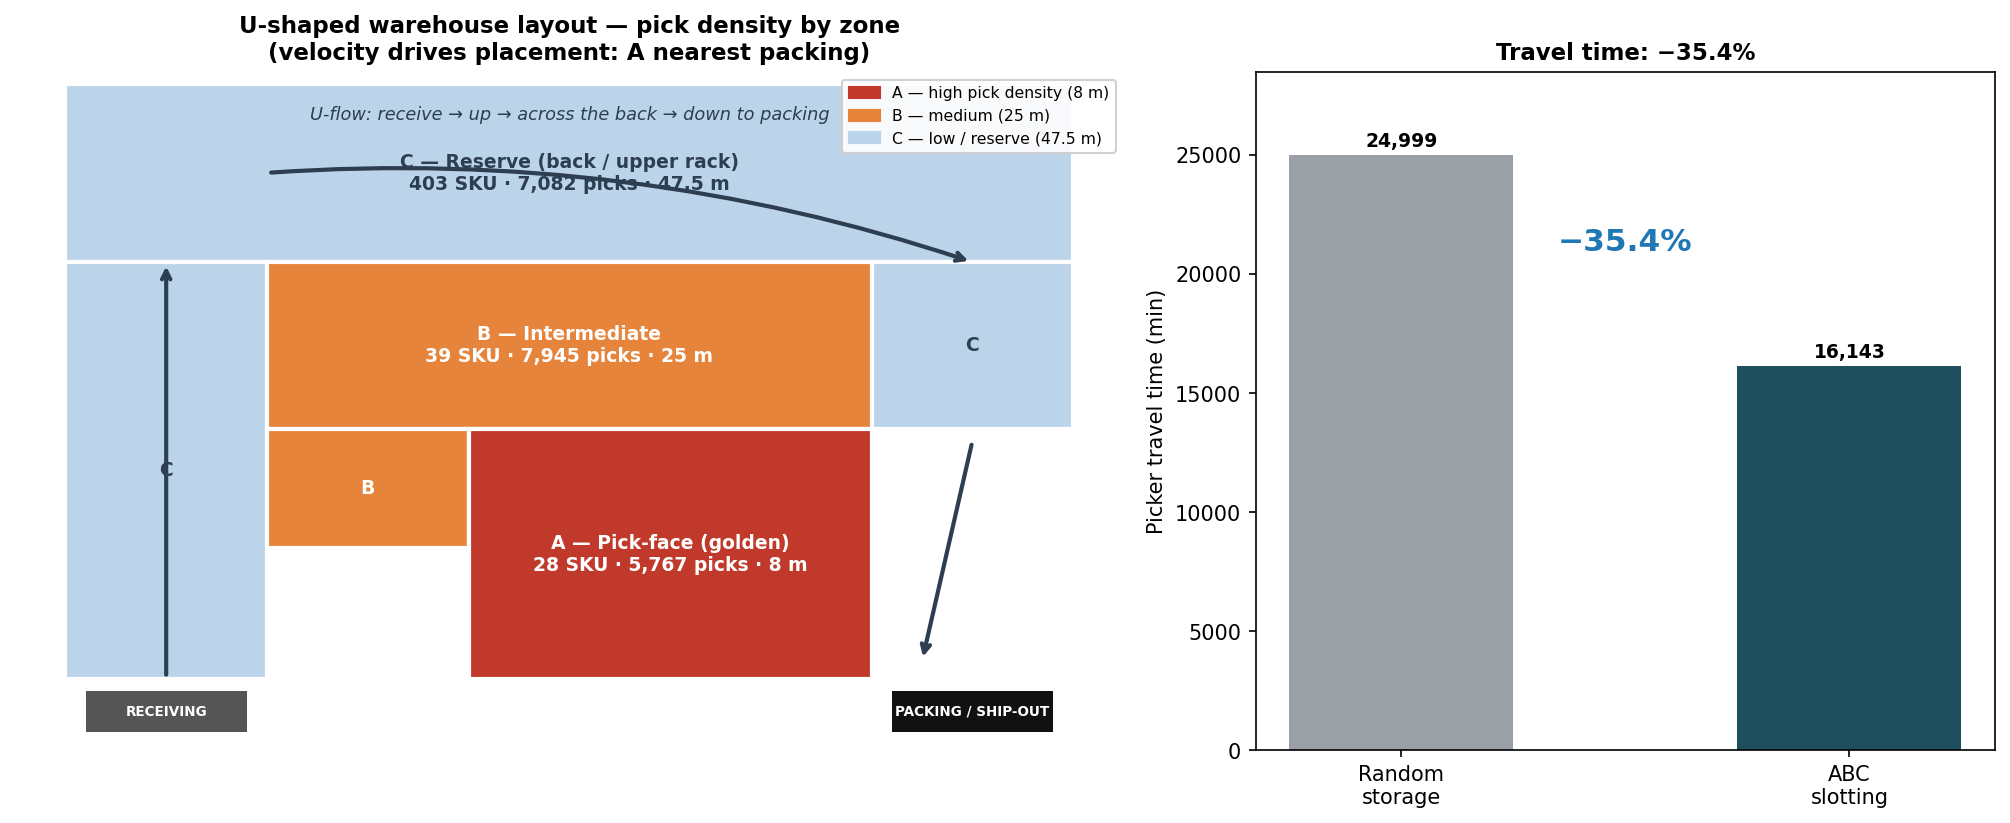
\includegraphics[width=0.75\linewidth]{../charts/q31_u_shape_heatmap.png}
\caption{U-Shaped Warehouse Heatmap --- ABC Velocity Zones}
\label{fig:q31-u-shape}
\end{figure}

\begin{itemize}
    \item \textbf{U-flow configuration}: Receiving and shipping docks share the same front wall;
          highest-frequency slots cluster at the dock end (Zone A golden pick-face).
    \item \textbf{Zone A --- Pick-Face (Ground Level)}: Class A SKUs at ergonomic height
          (lower rack levels), nearest the I/O dock and packing station.
          High-frequency Class AA SKUs occupy the first rank slots.
    \item \textbf{Zone B --- Forward Reserve}: Class B SKUs in the mid-bay area;
          two-bin replenishment logic feeds the Zone A pick-face (WMS-triggered min/max).
    \item \textbf{Zone C --- Reserve / Bulk}: Class C SKUs in upper racks and pallet block-stacks
          at the far back wall. Slow-movers are consolidated here; picked on demand.
\end{itemize}

\subsection{Question 3.2: Omni-Channel Pick-and-Pack Process Design}\label{q3.2}

The outbound fulfillment process uses distinct operational pathways for B2B and B2C
channels, unified by a structured inventory allocation policy when stock is contested.

\paragraph{Two pick models.}

\begin{table}[H]
\centering
\caption{Two Pick Models --- B2B vs B2C / E-Commerce}
\begin{tabular}{>{\raggedright\arraybackslash}p{1.8cm} >{\raggedright\arraybackslash}p{3.2cm} >{\raggedright\arraybackslash}p{3.2cm} >{\raggedright\arraybackslash}p{4.8cm} >{\raggedright\arraybackslash}p{2.8cm}}
\toprule
Channel & Order Profile & Pick Model & Mechanics & Pack \\
\midrule
        B2B & Large volume, few SKUs & Pallet / Total Picking & One picker fulfils whole pallets or large CTN qty per order in a single pass. Sources Zone A pick-face + Zone C bulk. & Stage whole pallets; minimal re-sort. \\\\
        \addlinespace
        B2C / E-com & Small qty, many SKUs, many concurrent orders & Batch Picking + Zone Routing & Group many small orders into one pick wave; pickers route by zone; items consolidated at sortation. & Sort wave back to individual orders at packing. \\\\
\bottomrule
\end{tabular}
\end{table}

\subsubsection{B2B Pathway — Pallet / Total Picking}\label{b2b-path}
\begin{enumerate}
    \item \textbf{Order release}: WMS validates on-hand stock against the B2B
          purchase order (contractual quantities and lead times).
    \item \textbf{Pick instruction}: Full-pallet or full-CTN pick task issued to operator.
    \item \textbf{Pick execution}: Operator uses forklift or reach truck to retrieve
          entire pallet(s) from the Forward Reserve Zone (B) or Reserve/Bulk Zone (C).
          Items bypass individual sortation.
    \item \textbf{B2B QC Station}: Wrap inspection, quantity verification, and
          outbound labeling.
    \item \textbf{Dispatch}: Pallets staged at outbound dock, loaded onto FTL truck.
\end{enumerate}

\subsubsection{B2C / E-Commerce Pathway — Batch Picking + Zone Routing}\label{b2c-path}
\begin{enumerate}
    \item \textbf{Batch wave release}: Multiple B2C orders are grouped into a single
          pick wave based on SKU proximity and delivery-window urgency.
    \item \textbf{Batch pick-to-cart}: Picker traverses Zone 1 (Pick-Face Zone) in a
          single pass with a multi-compartment cart, collecting all items for the wave.
    \item \textbf{Sort \& consolidate}: At the sortation station, items are separated
          by individual order and consolidated into shipment boxes.
    \item \textbf{QC + pack}: Bubble wrap or polybag packing, shipping label applied.
    \item \textbf{Dispatch}: Parcels handed to last-mile courier.
\end{enumerate}

\subsubsection{Stock Allocation Conflict and Escalation Policy}\label{conflict}

When the same SKU is ordered simultaneously by a B2B client and a B2C customer
and on-hand stock is insufficient for both, the system resolves the shortage through
the following structured rules (stock is held in ONE shared pool per the Q2.2 pooling strategy, not physically split):

\begin{table}[H]
\centering
\caption{Shared-SKU Conflict --- Allocation \& Escalation Rules}
\begin{tabular}{lp{4cm}p{6.5cm}}
\toprule
Rule & Condition & Action \\
\midrule
        Check & Same SKU, both channels, concurrent & Evaluate on-hand vs (B2B + B2C) demand. \\\\
        Sufficient & On-hand $\geq$ B2B + B2C & Allocate to both from shared pool; no rationing. \\\\
        R1 & Short stock & Commit to the confirmed B2B PO first (contractual, penalty risk). \\\\
        R2 & Short stock & Hold the B2C safety buffer so the storefront does not show stockout. \\\\
        R3 & Short + B2C SLA-critical (2--4\,h) & Split: B2C SLA order gets partial now, backorder remainder. \\\\
        R4 & Below reorder point & Trigger emergency replenishment / inter-warehouse transfer. \\\\
\bottomrule
\end{tabular}
\end{table}

Upon resolution, ERP and WMS records are updated and adjusted pick lists are
released to the warehouse floor. Figure \ref{fig:q32-flowchart} illustrates the
complete decision logic.

\begin{figure}[H]
\centering
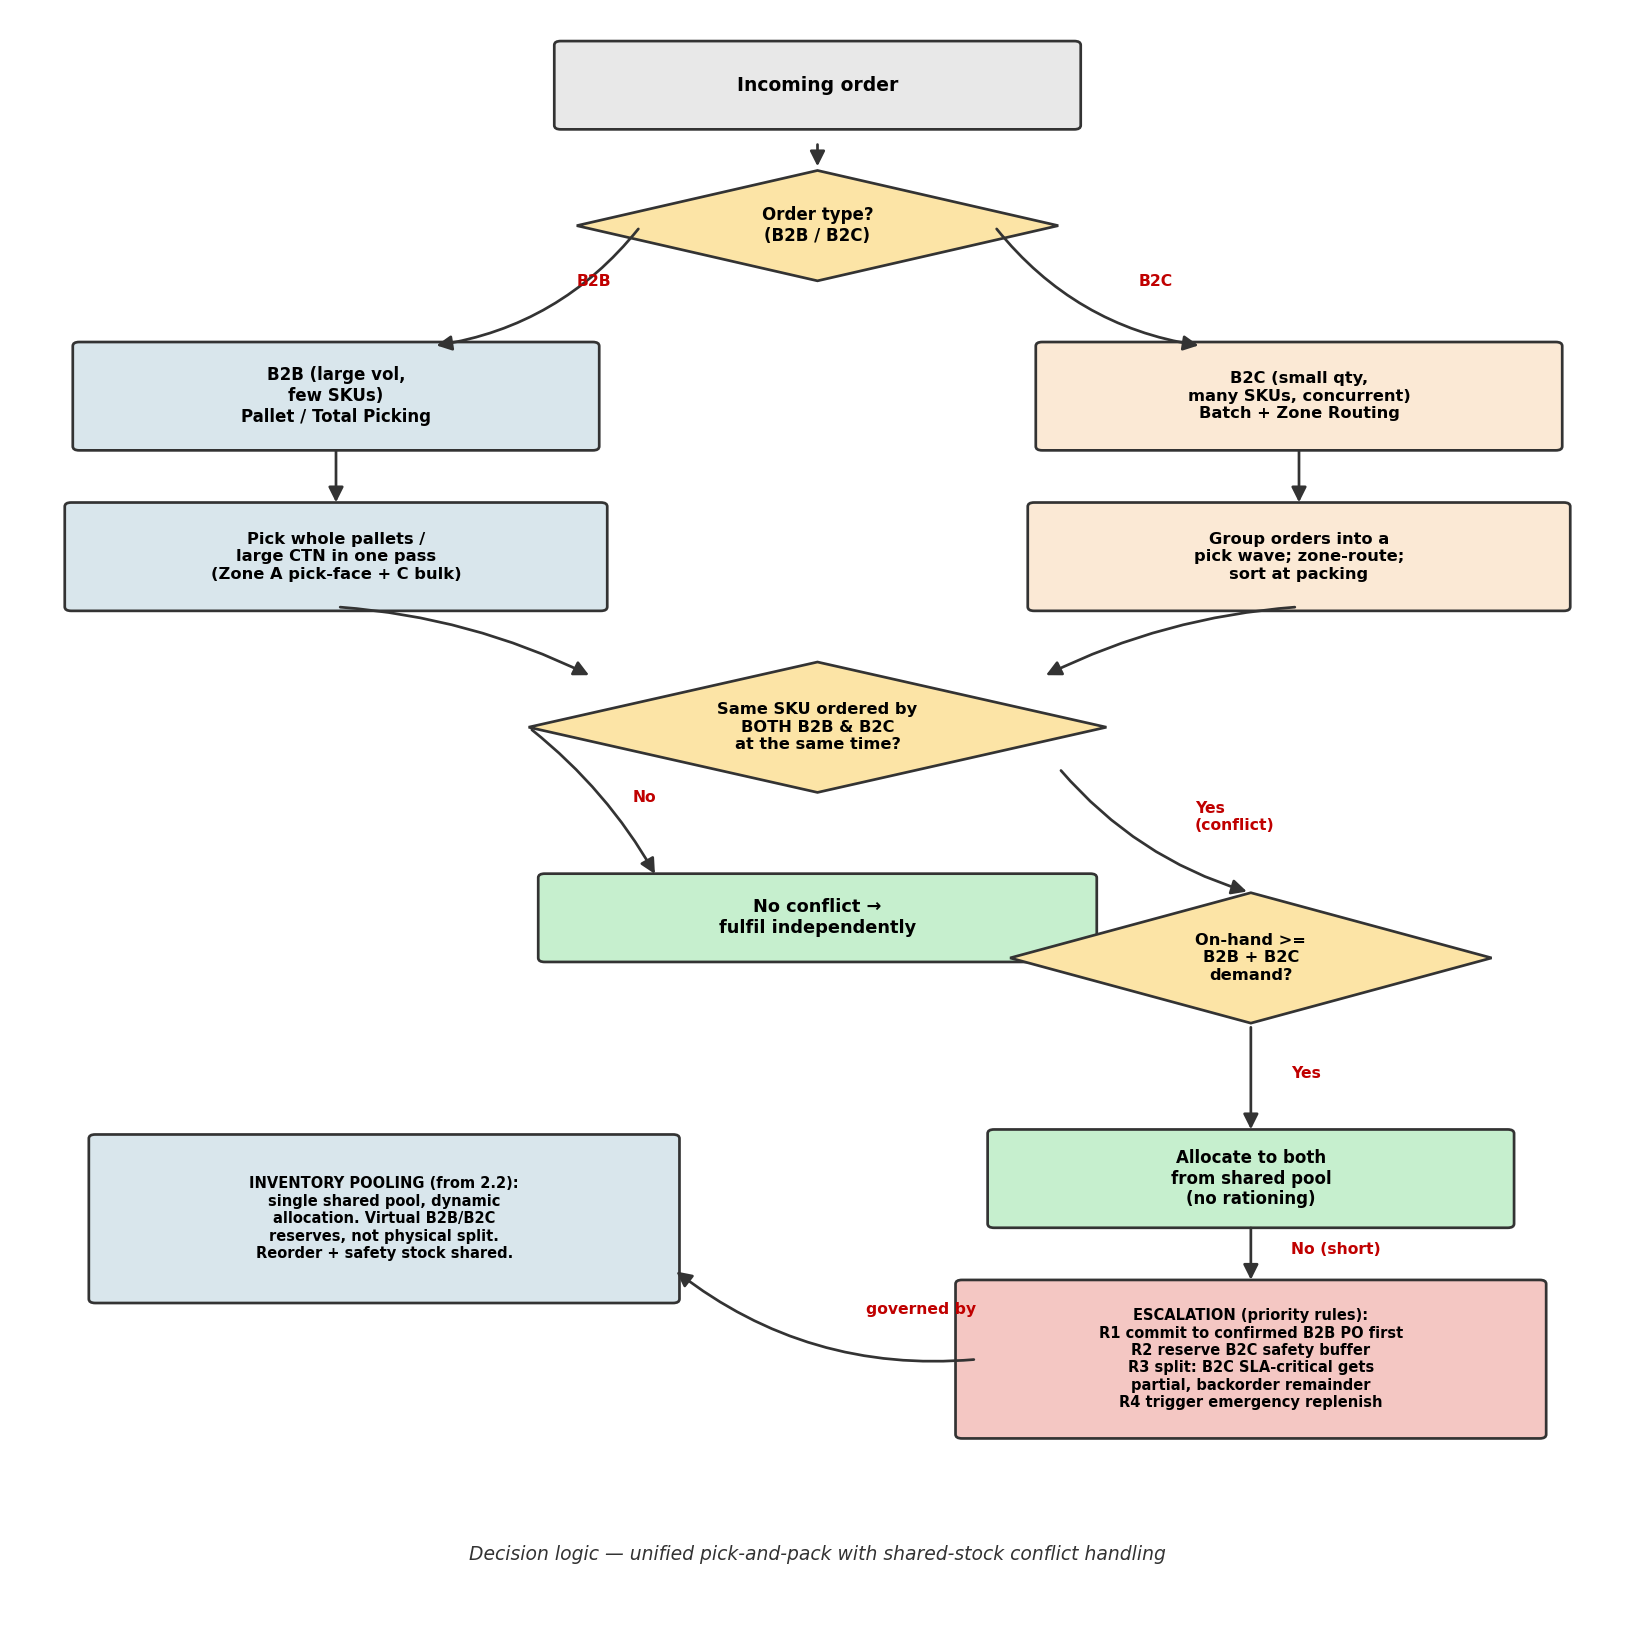
\includegraphics[width=0.88\linewidth]{../charts/q32_pick_pack_flowchart.png}
\caption{Q3.2 Omni-Channel Pick-and-Pack Process and Conflict Resolution Flowchart}
\label{fig:q32-flowchart}
\end{figure}

\end{document}
